\chapter{Garantovaný odhad parametrov}
V predošlej časti sme spomenuli niekoľko metód na odhad parametrov a každá si so sebou nesie určité nároky na namerané údaje. Napríklad taká metóda najmenších štvorcov predpokladá, že šum merania má normálne rozdelenie. Čo sa stane, ak tento predpoklad alebo ďalšie, ktoré sme uviedli v časti \aps{Požadavky na odhad parametrov}, nebude dodržaný ? Je zrejmé, že to povedie k nesprávnym výsledkom. 

Zostáva tu však ešte jeden problém, ktorý je omnoho zložitejší ako samotný odhad parametrov, a tým je voľba štruktúry dátového modelu. Pomocou metódy najmenších štvorcov môžeme odhadovať parametre modelu ľubovoľnej štruktúry, v prípade že je zabezpečená linearita. Ale ako zistíme, či daný model nezanedbáva dôležitú časť dynamiky procesu alebo na druhej strane, či už neaproximuje šum merania ? Riešenie môže ponúknuť práve metóda garantovaného odhadu parametrov.

Garantovaný odhad parametrov (GOP) je metóda, ktorá obchádza problém poznania rozdelenia náhodných veličín a namiesto toho predpokladá ľubovoľnú ale ohraničenú chybu merania. Výsledkom identifikácie pomocou GOP sú intervalové odhady parametrov modelu, ktoré zabezpečia, že nameraný výstup procesu sa bude nachádzať v rozmedzí stanovenej chyby merania \cite{paulen:gpe:2017}. Demonštrujme si fungovanie tejto metódy na nasledujúcom príklade.

\textbf{Príklad}
\newline
Predstavme si, že sme získali vstupné $ u $ a výstupné $ y $ údaje z procesu, ktoré v tomto prípade budú predstavovať konštantnú funkciu, tak ako to je zobrazené na Obr. \ref{gpe_ex1_data}. Vieme, že senzor má stanovenú chybu merania $ e $. Štruktúru modelu procesu, z ktorého sme získali údaje, nepoznáme a preto sa rozhodneme, že budeme tieto údaje aproximovať lineárnym modelom
\begin{equation}
	\hat{y}(u) = \theta_1 + \theta_2u.
\end{equation}
 Jediné neznáme v tomto modely sú parametre $ \theta_1 $ a $ \theta_2 $. Na ich identifikáciu využijeme grafickú metódu GOP a začneme tým, že si vyjadríme parameter $ \theta_2 $ ako funkciu nameraných údajov $ y, u $ a parametra $ \theta_1 $
\begin{equation} \label{gpe:ex_lin_model}
	\theta_2 = \frac{1}{u}y - \frac{1}{u}\theta_1,
\end{equation}
kde $ \theta_2 $ teraz predstavuje nezávislú premennú a $ \theta_1 $ závislú. Cieľom odhadu parametrov bude, aby ich vzájomná kombinácia viedla k výstupným údajom modelu $ \hat{y}(u) $, ktoré budú ležať v rozmedzí hraníc chyby merania senzora. Táto podmienka upravuje rovnicu \ref{gpe:ex_lin_model} do tvaru
\begin{equation} 
	\theta_2 = \frac{1}{u}\left(y \pm e\right) - \frac{1}{u}\theta_1,
\end{equation}
ktorú môžeme formálne rozpísať na dve rovnice 
\begin{equation}
	\begin{split}
		\theta_2^{(1)} =& \frac{1}{u}\left(y + e\right) - \frac{1}{u}\theta_1,\\
		\theta_2^{(2)} =& \frac{1}{u}\left(y - e\right) - \frac{1}{u}\theta_1.
	\end{split} 
\end{equation}
Tieto priamky vytyčujú oblasť vhodných kombinácií parametrov modelu $ \theta_1, \theta_2 $ ktorými môžeme opísať dané dáta a garantuje, že správne riešenie leží niekde vo vnútri tejto oblasti.

\begin{figure}
	\centering
	\begin{subfigure}[b]{0.48\textwidth}
		\centering
		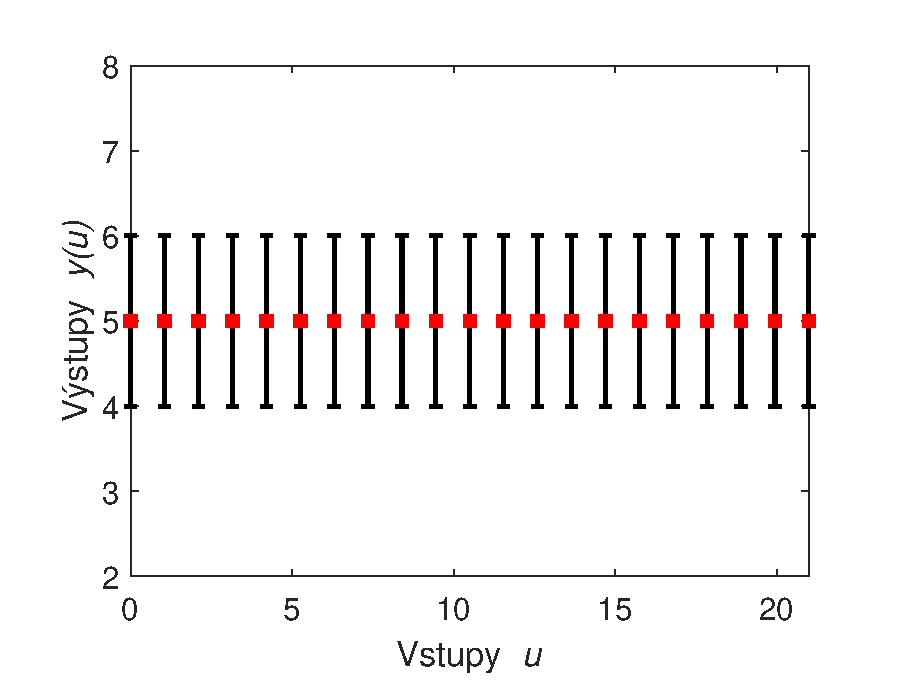
\includegraphics[width=\linewidth]{images/gpe_ex_data1}
		\caption{Namerané výstupné údaje z neznámeho procesu.}
		\label{gpe_ex1_data}
	\end{subfigure}
	\begin{subfigure}[b]{0.48\textwidth}
		\centering
		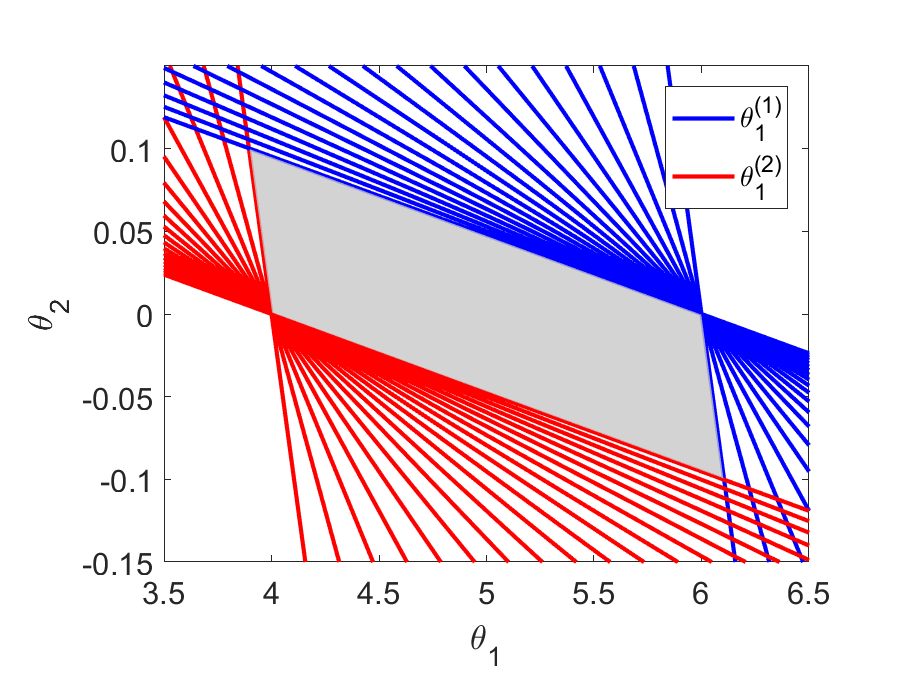
\includegraphics[width=\linewidth]{images/gpe_ex_line1}
		\caption{Grafická metóda garantovaného odhadu parametrov.}
		\label{gpe_ex1_gm}
	\end{subfigure}
	\caption{Ilustračný príklad garantovaného odhadu parametrov -- variant 1 -- zidealizovaný prípad.}
	\label{gpe_ex1}
\end{figure}

Takto sme získali nielen informácie o parametroch nášho modelu, ale aj informácie o zložitosti resp. jednoduchosti štruktúry modelu. Na Obr. \ref{gpe_ex1_gm} vidíme, že parameter $ \theta_2 $ obsahuje vo svojom intervale nulu, čím sa porušuje invariantnosť štruktúry modelu a môžeme tvrdiť, že takýto matematický opis je potenciálne zbytočne zložitý. Rovnaké dáta by sme teda vedeli opísať aj konštantným modelom, t.j. 
\begin{equation}
	\hat{y}(u) = \theta_1.
\end{equation}

 Avšak dáta zobrazené na Obr. \ref{gpe_ex1} boli trošku zidealizované a pravdepodobne v bežnom živote by nenastala situácia, že by senzor niekoľkokrát po sebe nameral tú istú hodnotu. Pozrime sa však, čo sa stane, ak naše namerané údaje budú mať bližšie k realite, tak ako je uvedené na Obr. \ref{gpe_ex2_data}. Ako si môžeme všimnúť na Obr. \ref{gpe_ex2_gm}, odhadované ohraničenie jednotlivých parametrov $ \theta_1, \theta_2 $ sa nám výrazne zmenšilo. Takže môžeme tvrdiť, že samotný šum merania nám prispieva k presnosti odhadu parametrov. 

\begin{figure}
	\centering
	\begin{subfigure}[b]{0.48\textwidth}
		\centering
		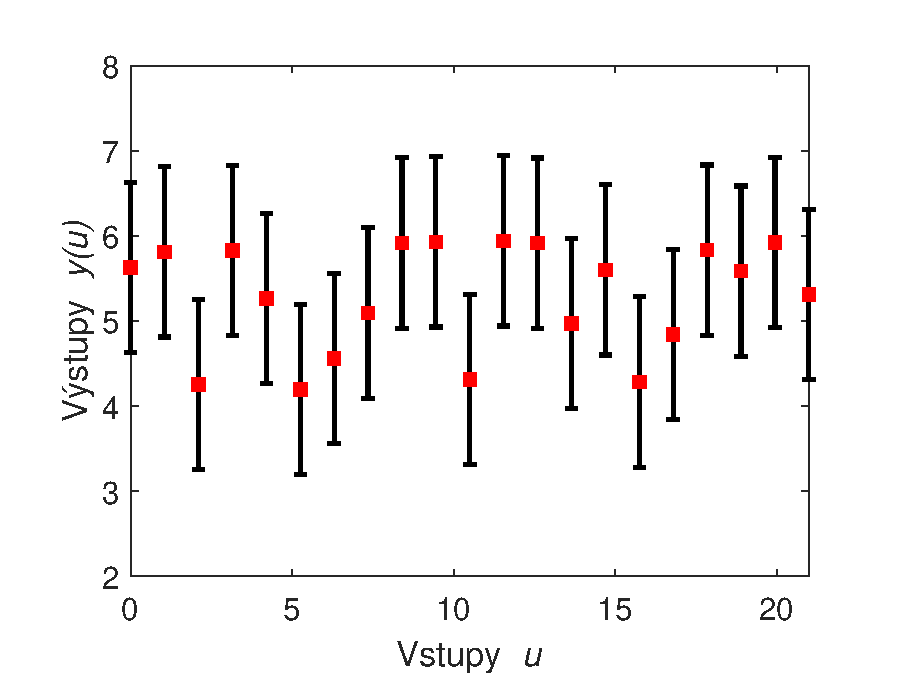
\includegraphics[width=\linewidth]{images/gpe_ex_data2}
		\caption{Namerané výstupné údaje z neznámeho procesu.}
		\label{gpe_ex2_data}
	\end{subfigure}
	\begin{subfigure}[b]{0.48\textwidth}
		\centering
		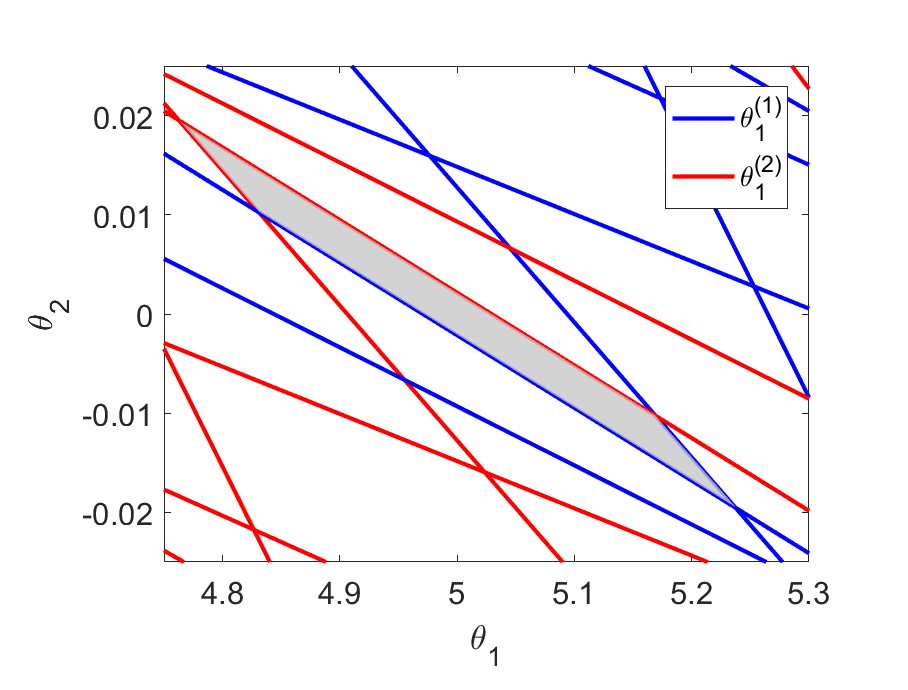
\includegraphics[width=\linewidth]{images/gpe_ex_line2}
		\caption{Grafická metóda garantovaného odhadu parametrov.}
		\label{gpe_ex2_gm}
	\end{subfigure}
	\caption{Ilustračný príklad garantovaného odhadu parametrov -- variant 2.}
	\label{gpe_ex2}
\end{figure}

\section{Odhad parametrov FIR modelu}

\section{Odhad parametrov ARX modelu}

